%\usepackage{graphics}
%\setlength{\hoffset}{-0.5in} \setlength{\oddsidemargin}{0.5in}
%\setlength{\textwidth}{6.5in} \setlength{\textheight}{8.7in}
%\usepackage[total={6.5in,8.75in}
%\usepackage{geometry}


\documentclass[12pt,english]{report}
%%%%%%%%%%%%%%%%%%%%%%%%%%%%%%%%%%%%%%%%%%%%%%%%%%%%%%%%%%%%%%%%%%%%%%%%%%%%%%%%%%%%%%%%%%%%%%%%%%%%%%%%%%%%%%%%%%%%%%%%%%%%
\usepackage{amssymb,amsthm,amsmath}
\usepackage[spanish,activeacute]{babel}
\usepackage{graphics}
\usepackage{graphicx}
\usepackage[total={6.5in,8.75in},top=1.2in, left=0.9in, includefoot]{geometry}

\setcounter{MaxMatrixCols}{10}
%TCIDATA{OutputFilter=Latex.dll}
%TCIDATA{Version=4.00.0.2321}
%TCIDATA{LastRevised=Thursday, June 07, 2007 13:17:06}
%TCIDATA{<META NAME="GraphicsSave" CONTENT="32">}

\newtheorem{theorem}{Teorema}[section]
\newtheorem{corollary}{Corolario}[theorem]
\newtheorem{lemma}[theorem]{Lema}
\newtheorem{proposition}{Proposici\'{o}n}[section]
\newtheorem{remark}{Observaci\'{o}n}[section]
\newtheorem{example}{Ejemplo}[section]
\newtheorem{definition}{Definici\'on}[section]
\newtheorem{claim}{Criterio}[section]
\renewcommand{\baselinestretch}{1.1} 
\newtheorem{conjecture}[theorem]{Presupuesto}


\begin{document}


%\title{Crecimiento y decrecimineto de pol\'igonos mediante paralelas.}
%\author{Nelson Gonz\'{a}lez Jhones}


\title{Crecimiento y decrecimineto de pol\'igonos mediante paralelas.}
\author{Nelson Gonz\'{a}lez Jhones}
\maketitle

\pagestyle{empty}
\chapter*{Dedicatoria}
A mi madre.

%\newpage
\chapter*{Agradecimientos}

A Pablo por haberme ayudado en toda la carrera.

A Tony por darme la posiblidad de trabajar con \'el.

A Eduardo por su dedicaci\'on.

\newpage

\begin{center}
\textbf{Resumen}
\end{center}

En este trabajo se expone un m\'etodo sencillo para el ensanchamiento o encogimiento de pol\'igonos en el plano. Se hace un an\'alisis de la complejidad que se presenta en el mismo cuando son localmente tratadas las intersecciones producidas con el aumento de la distancia. Se realiz\'o una sencilla implementaci\'on de algoritmo de construcci\'on del esqueleto recto de un pol\'igono simple. Se brinda, adem\'as, un algoritmo construye el apropiado conjunto de pol\'igonos resultante de este problema a partir de esta estructura.



\tableofcontents

\pagestyle{plain}
\setcounter{secnumdepth}{-1}
\chapter{Introducci\'on}  

 El prop\'osito de este trabajo de diploma es dar soluci\'on al problema de hacer crecer o decrecer un pol\'igono simple $P$ mediante paralelas, habiendo fijado previamente, una distancia. Esto equivale a la realizaci\'on de un apropiado proceso de contracci\'on o dilataci\'on de $P$ hasta obtener el apropiado conjunto de pol\'igonos resultante.
 
   
En la pr\'actica,  se pueden encontrar varias aplicaciones de este problema, como por ejemplo, en el c\'alculo del techo de un edificio dada la geometr\'ia que forman sus paredes en una vista a\'erea. 

En la literatura que comprende el campo de la geometr\'ia computacional es conocido un problema similar. Este problema consiste en hacer crecer o decrecer un pol\'igono manteniendo fija una distancia a su frontera. El resultado de esto da lugar a curvas parab\'olicas en las vecindades de un v\'ertice reflexivo (v\'ertice cuyas aristas incidentes forman un \'angulo mayor que $\pi$ en el interior del pol\'igono). En el resultado del problema tratado en este trabajo, esto no es deseado, por el contrario se especifica mantener un n\'umero acotado de segmentos los cuales tienen un correspondiente paralelo en el pol\'igono original.  

A lo largo de este trabajo se expondr\'a una serie de particularidades que trae consigo este problema. Estas ponen en evidencia la complejidad del mismo. Primeramente ser\'a abordada una v\'ia directa en pro de lograr su soluci\'on. Con esta, no todos los casos fueron resueltos. Esta es la raz\'on por la cual, a pesar de que esta v\'ia se deja propuesta para una futura investigaci\'on, el estudio del problema fue dirigido en otra direcci\'on. 

En el cap\'itulo $2$ es estudiada una estructura poco conocida, el esqueleto recto de un pol\'igono simple. Tambi\'en en este cap\'itulo, se reflejan algunas de las propiedades de esta estructura que justifican el porqu\'e de su uso en el tratamiento del problema presentado. Se brindan, adem\'as, los detalles de una sencilla implementaci\'on del algoritmo de construcci\'on de esta estructura. 

Finalmente es presentado un algoritmo que computa, a partir del esqueleto recto, el adecuado conjunto soluci\'on del objetivo trazado.

%%%%%%%%%%%%%%%%%%%%%%%%%%%%%%%%%%%%%%% Fin de la introducion

%%%%%%%%%%%%%%%%%%%%%%%%%%%%%%%%%%capitulo de invertidos
\setcounter{secnumdepth}{2}
\chapter{Una forma de abordar el problema}

El problema que intentamos resolver consiste en hacer crecer o decrecer un pol\'igono $P$ habiendo fijado, previamente, una distancia $d$. El resultado de esta operaci�n est\'a dado por un conjunto de poligonales cerradas. Ver Figura 1.1. En lo adelante nos referiremos a este conjunto como poligonal resultante $P'$.   

\begin{figure}[htbp]
\begin{center}
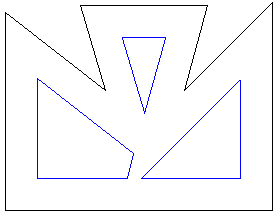
\includegraphics{conjunto.jpg}%[width=15cm]
\end{center}
\caption{Resultado del encogimeinto de un pol\'igono mediante paralelas.}
\end{figure}

A cada segmento de $P'$ le corresponde un \'unico segmento del pol\'igono original $P$. Esto no ocurre en sentido contrario, no necesariamente a todo segmento de $P$ le corresponde un segmento de $P'$. Esta relaci\'on viene dada de la siguiente manera. Sean los segmentos $s$ y $s'$ tal que $s \in P$ y $s' \in P'$. Si $s$ es el segmento correspondiente de $s'$, entonces se cumple que $s'$ es paralelo a $s$ y la distancia entre ellos es $d$.

Geom\'etricamente el resultado de hacer crecer (decrecer) un pol\'igono $P$ mediante paralelas a una distancia $d$ puede ser visto al intentar dibujar $P$ con una pluma de grosor $d$. %Ver Figura 1.2. 

\begin{figure}[h]
\begin{center}
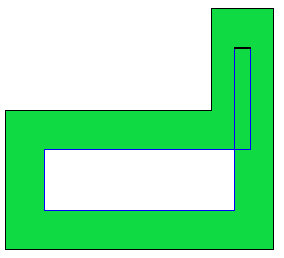
\includegraphics{pluma.jpg}%[width=15cm]htbp
\end{center}
\caption{Resultado de trazar por sobre la frontera de $P$ una pluma de grosor $d$.}
\end{figure}

El proceso de trazar una l\'inea paralela a cada arista de $P$ a distancia $d$, estableciendo una correspondencia uno a uno, as\'i como el c\'alculo de las intersecciones con sus aristas adyacentes es simple. El resultado de este proceder consiste en una poligonal cerrada $P'$ que a diferencia de $P$ no tiene que ser simple. Ver Figura 1.3(a).

\begin{figure}[htbp]
\begin{center}
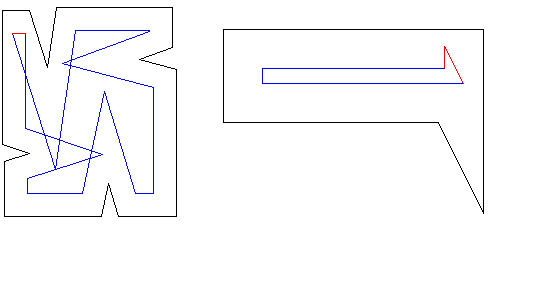
\includegraphics{tonyza.jpg}%[width=15cm]
\end{center}
\caption{(a) $P'$ no es simple y (b) otras consecuencias no deseables.}
\end{figure}

El aumento de la distancia trae m\'ultiples consecuencias no deseables en el resultado. Una de ellas es que puede cambiar la geometr\'ia del pol\'igono resultante con respecto a la del original. Ver Figura 1.3(b). 


Este aumento da lugar tambi\'en a la aparici\'on de regiones en el resultado producto de intersecciones entre segmentos no adyacentes. Estas regiones pudieran ser no deseables. Ver Figura 1.2. En la analog\'ia expuesta, esto se evidencia como el solapamiento del trazo de grazor $d$ por sobre dos segmentos no adyacentes. Ver Figura 1.2.

Si se lograse diferenciar cuando una regi\'on es deseable o no, se tendr\'ia una v\'ia de soluci\'on al problema ya que los casos, similares al mostrado en la Figura 1.3(b), pueden ser localmente tratados en la construcci�n de $P'$. Bastar\'ia con eliminar toda regi\'on no deseable y obtener el resto como resultado. A continuaci\'on se expondr\'an algunas ideas analizadas con vistas a lograr dicho objetivo. 

\section{La idea del Plane-Sweep} 

Para diferenciar las regiones primero tenemos que hallarlas. Como ya se ha visto, las regiones estar\'an dadas por intersecciones de segmentos en el plano. Por tal motivo se hizo uso de la t\'ecnica del plane-sweep siguiendo la idea usada para resolver el problema de determinar las intersecciones de $n$ segmentos en un plano. Sin embargo esto no es suficiente ya que, no s\'olo es necesario determinar las regiones, sino tambi\'en clasificarlas. 

En el mismo momento en que se identifique una regi\'on, esta ser\'a clasificada. La base de esto \'ultimo est\'a sustentada en los siguientes lemas. \\
     

\noindent Sea $C$ una curva cerrada y orientada en el plano, que divide al plano en $k$ regiones diferentes.

\begin{lemma}
Sean $r_{1}$ y $r_2$ dos rayos que van desde los puntos $x_1$ y $x_2$ respectivamente, hasta el infinito. Si $x_1$ y $x_2$ pertenecen a una misma regi\'on determinada por $C$, entonces la diferencia entre los cortes de izquierda a derecha y los cortes de derecha a izquierda de $C$ con $r_1$ y $r_2$ ser\'a la misma.
\end{lemma}

\begin{proof}
Sea $z$ una curva orientada que pase por los puntos $x_1$ y $x_2$. Sup\'ongase que se realiza dos recorridos sobre $z$ a partir de los puntos $x_1$ y $x_2$ en sentidos contrarios. Sean $d_1$ y $i_1$ los cortes derecha a izquierda y los cortes de izquierda a derecha respectivamente, de $z$ con $C$ en el recorrido a partir de $x_1$. Sim\'etricamente $d_2$ y $i_2$ representan los cortes del recorrido a partir de $x_2$. Sup\'ongase adem\'as, que entre $x_1$ y $x_2$, $z$ no corta a $C$. Entonces se cumple que $d_1 + i_2 = d_2 + i_1$ ya que $C$ es cerrada y por tanto $d_1 - i_1 = d_2 - i_2$. 

En particular, los recorridos a partir de $x_1$ y $x_2$ pueden ser rectos y con esto queda terminada la demostraci\'on.
\end{proof}

Es posible establecer un sentido a $P'$. Sup\'ongase los v\'ertices del pol\'igono $P'$ y sus aristas orientadas en contra de las manecillas del reloj. As\'i pues, $P'$ puede verse como una poligonal cerrada orientada en el plano.

T\'engase una recta vertical $r$ y un entero $t$, inicialmente con valor cero, asociado a la misma. La recta $r$ se desplazar\'a horizontalmente cubriendo todo el plano y $t$ ser\'a modificado de la siguiente manera:

\begin{itemize}
	\item[$\triangleright$] $t := t - 1$ si $r$ corta a $P'$ de izquierda a derecha
	\item[$\triangleright$] $t := t + 1$ si $r$ corta a $P'$ de derecha a izquierda  
\end{itemize}

As\'ignesele a cada regi\'on el valor de $t$.  Un segmento de $P'$ formar\'a parte de una regi\'on deseable si tiene una regi\'on adyacente con valor $-1$ y otra con valor $0$. El \textbf{Lema 1.1.1} asegura que, independientemente del camino por el cual se llegue a una regi\'on, esta siempre tendr\'a el mismo valor.

El problema presente es que hay inicialmente regiones de $P'$ inexistente en relaci\'on a la comparaci\'on geom\'etrica entre $P'$ y $P$. Ver Figura 1.4. Estas regiones deber\'ian ser eliminadas puesto que no tiene sentido clasificarlas. Adem\'as de esto, estas pueden presentar conflicto en la adecuada clasificaci\'on de otras regiones ya que podr\'ia intersectarlas. De esta forma se originar\'ian nuevas regiones tambi\'en inexistentes. 

\begin{figure}[htbp]
\begin{center}
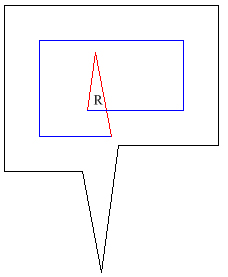
\includegraphics{pico1.jpg}%[width=15cm]
\end{center}
\caption{$R$ regi\'on inexistente y segmentos invertidos representados en rojo}
\end{figure}

En la pr\'oxima secci\'on se analiza una caracter\'istica com\'un de este tipo de regiones. Dicha caracter\'istica ser\'a utilizada para su previa detecci\'on. Se propone, adem\'as, una secuencia de criterios para la eliminaci\'on apropiada de las mismas.

\section{\textquestiondown Criterios o conjeturas?}

Se entender\'a por \emph{segmento invertido} de $P'$ aquel cuyo sentido se encuentra en oposici\'on con su correspondiente en $P$. Recu\'erdese que se ha establecido una orientaci\'on a los segmentos de $P$. Ver Figura 1.4.\bigskip

Un segmento invertido aislado representa un segmento que, a la distancia dada, no deber\'ia reflejarse en $P'$. Ver Figura 1.4. Una secuencia de segmentos invertidos puede generar regiones no deseables. Consecuentemente con la eliminaci\'on de los segmentos invertidos son eliminadas las regiones que estos conforman. Se realiz\'o un estudio en b\'usqueda de un apropiado m\'etodo para la eliminaci\'on de estos segmentos. El m\'etodo se encuentra basado en los tres criterios siguientes.

\begin{claim}
Si en el resultado se encuentra una cadena de segmentos invertidos de
longitud mayor que dos, entonces son eliminados todos los segmentos de la cadena
excepto el primero y \'{u}ltimo. Se obtiene de esta forma, un par de segmentos
invertidos que pudieran o no intersectarse.
\end{claim}

\begin{claim}
Si tenemos un segmento invertido aislado, significa que, a la distancia dada, ese
segmento no debe verse reflejado en el resultado. En consecuencia de esto, es
eliminado y es hallada la intersecci\'{o}n (si existe) entre los segmentos
adyacentes a este. La consecuencia de esta intersecci\'on, sobre los mismos, es analizada en ese momento.
\end{claim}

\begin{claim}
Teniendo un par de segmentos invertidos, no eliminar aquel que luego de la
eliminaci\'{o}n de su adyacente invertido deje de serlo. En caso de que esto
sea imposible eliminamos a ambos, por otra parte en el caso de tener
reflexividad no llegamos a contar con un criterio s\'{o}%
lido sobre cual de los dos segmentos debiera eliminarse.
\end{claim}        

En cualquiera de los criterios anteriores pudiera suceder que la intersecci\'on del nuevo par de segmentos adyacentes no invertidos no existiera (los segmentos son paralelos). En este punto  es analizada la eliminaci\'on de uno o de ambos, sim\'etricamente a la manera en que se procede a la eliminaci\'on de segmentos invertidos.

Este proceso no es incremental en la reducci\'on del n\'umero de segmentos invertidos. Debido a las nuevas intersecciones que se producen, segmentos que en principio no eran invertidos pudieran llegar a serlo. 

Por lo antes expuesto el punto de parada del proceso de decremento del n\'umero de segmentos invertidos, no est\'a dado por la eliminaci\'on local de un segmento invertido. Este se encuentra en la eliminaci\'on global de los segmentos invertidos de la poligonal resultante, puesto que el n\'umero de segmentos en ella, es finito. 

Luego de la aplicaci\'on de los criterios vistos, las regiones inducidas por los segmentos invertidos pasan a eliminarse. Desafortunadamente la eliminaci\'on de estos segmentos trae como consecuencia la generaci\'on de nuevas regiones en $P'$. Estas nuevas regiones son inexistentes en el sentido analizado y, a diferencia de las conformadas por segmentos invertidos, cumplen una caracter\'istica. Esta caracter\'istica est\'a dada entre un par de segmentos adyacentes que conforman dicha regi\'on y se encuentra determinada por lo siguiente: \textit{La posici\'on relativa entre un par de segmentos no invertidos adyacentes en  $P'$ difiere a la posici\'on relativa entre sus correspondientes no adyacentes en $P$}. Ver Figura 1. 


\begin{figure}[htbp]
\begin{center}
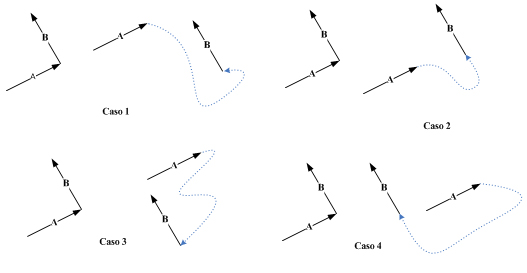
\includegraphics{casos1.jpg}%[width=15cm]
\end{center}
\caption{En el \textbf{Caso 1} B est\'a invertido , en el \textbf{Caso 2} ninguno de los dos est\'an invertidos, en el \textbf{Caso 3} ambos est\'an invertidos y en el \textbf{Caso 4} A est\'a invertido.}
\end{figure}

Esto formar\'a parte del m\'etodo por lo que se expone en un cuarto criterio.  

\begin{claim}
Teniendo un par de segmentos $s_1$ y $s_2$ consecutivos en $P'$, que no lo son en $P$. Si $s_1$ est\'a a la izquierda (a la derecha) de $s_2$ en $P'$ y $s_1$ se encuentra a la derecha (a la izquierda) de $s_2$ en $P$ entonces $s_1$ es considerado como invertido por este criterio. Sim\'etricamente es analizada la posici\'on de $s_2$ respecto a $s_1$.
\end{claim} 

Luego que de ser calculada una nueva intersecci\'on es aplicado este \'ultimo criterio el cual, a lo sumo, da lugar al an\'alisis de la eliminaci\'on de dos segmentos. Esta eliminaci\'on es tratada consecuentemente con los tres primeros  criterios para segmentos invertidos.
 
Las regiones no deseables e inexistentes fueron eliminadas por un m\'etodo basado en estos criterios. En la pr\'oxima secci\'on se ver\'an los resultados arrojados por el trabajo realizado en esta direcci\'on.  

\section{Conclusiones y problemas abiertos}

El m\'etodo expuesto es muy eficiente y arroja resultados satisfactorios para distancias peque\~nas. Sin embargo, a pesar de la eliminaci\'on de las regiones no deseables, en algunos casos el resultado, de acuerdo con la especificaci\'on, fue inaceptable. El producto de la eliminaci\'on de segmentos localmente trae como consecuencia la eliminaci\'on de segmentos que deber\'ian aparecer en la poligonal resultante.

Las regiones o segmentos resultantes de la prolongaci\'on de los picos que son cortados completamente por alg\'un segmento de la poligonal original no deber\'ian tener consecuencias luego del corte. Ver Figura 1.6. Una v\'ia para detectar este problema, ser\'ia hacer un preprocesamiento con las aristas que forman los picos y las intersecciones, de estos, con la poligonal. Este proceso podr\'ia llevarse acabo usando la t\'ecnica del Plane-Sweep para detectar dichas intersecciones. Se ha utilizado la palabra completamente debido a que, si $P$ los hubiera cortado parcialmente, estos deber\'ian continuar con su prolongaci\'on, ver Figura 1.7. Este detalle tendr\'ia que tenerse en cuenta en la implementaci\'on. 

\begin{figure}[htbp]
\begin{center}
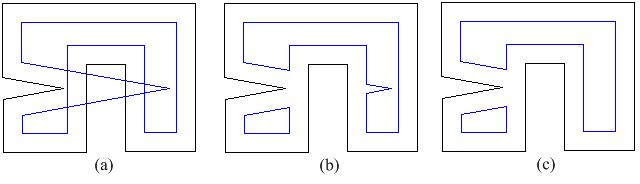
\includegraphics{comp2.jpg}%[width=15cm]
\end{center}
\caption{(a) Resultado directo de hacer la paralela a cada segmento, (b) resultado de la eliminaci\'on de las regiones no deseables y (c) resultado de la especificaci\'on.   }
\end{figure}

\begin{figure}[htbp]
\begin{center}
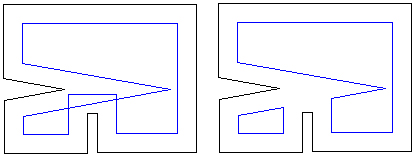
\includegraphics{parcial.jpg}%[width=15cm]
\end{center}
\caption{Corte parcial con el pol\'igono original }
\end{figure}

En el pr\'oximo cap\'itulo es analizada una soluci\'on indirecta del problema haciendo uso de una estructura auxiliar. Esta estructura permite realizar, de forma discreta, el crecimiento o decrecimiento de un pol\'igono. Esta operaci\'on se llevar\'a a cabo hasta que ocurra la primera intersecci\'on (entre segmentos no adyacentes) para entonces resolver el problema en esta situaci\'on y continuar recursivamente el proceso hasta alcanzar la distancia requerida. Esta v\'ia de soluci\'on permite identificar si un segmento del pol\'igono original tendr\'a o no un correspondiente en la poligonal resultante. 

%%%%%%%%%%%%%%%%%%%%%%%%%%%%%%%%%%Fin del capitulo de invertidos

%%%%%%%%%%%%%%%%%%%%%%%%%%%%%%%%%%Inicio de esqueleto

\chapter{El esqueleto recto}

Un grafo plano de l\'{\i}neas rectas $G$, sobre $n$ puntos en el plano
Euclidiano, es un conjunto de segmentos que no se cortan cubriendo todos
puntos del plano. Un esqueleto de $G$ es una partici\'{o}n del plano en
regiones de forma tal, que, cada regi\'{o}n refleja, de manera apropiada, la
forma geom\'{e}trica de $G$.

Entre los ejemplos m\'{a}s conocidos y ampliamente usados de esquetos se
encuentra el diagrama de Voronoi de $G$ o, si $G$ es un pol\'{\i}gono
simple, el eje medio o medial axis de $G$. Estos esqueletos quedan definidos
por todos los puntos del plano (pol\'{\i}gono en el caso del eje medio) que
tienen m\'{a}s de un elemento en $G$ m\'{a}s cercano. Es posible encontrar n%
\'{u}merosas aplicaciones de esqueletos tanto dentro como fuera del campo de
la ciencia de la computaci\'{o}n, por ejemplo en biolog\'{\i}a, geograf\'{\i}%
a, reconocimiento de patrones, rob\'{o}tica y gr\'{a}ficos por computadora.

\section{\textquestiondown Qu\'{e} es el esqueleto recto?}

En 1995 Aichholzer y Aurenhammer introducen un nuevo tipo de esqueleto para
pol\'{\i}gonos simples en el plano, el esqueleto recto. Este se encuentra
definido por el rastro que dejan los v\'{e}rtices del pol\'{\i}gono inicial
cuando este se ve encogido o ensanchado, movi\'{e}ndose de cada una de sus
aristas a una misma velocidad. Ver Figura 2.1(a).

\begin{figure}[htbp]
\begin{center}
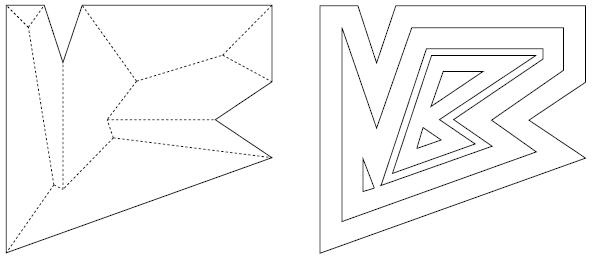
\includegraphics{jerar.jpg}
\end{center}
\caption{(a) Esqueleto recto y (b) jerarqu\'ia de pol\'igonos.}
\end{figure}

Sea $P$ un pol\'{\i}gono simple y $S(P)$ el esqueleto recto correspondiente
a $P$. Cada arco de $S(P)$, estar\'{a} formado por un segmento de la
bisectriz definida por un par de aristas de $P$. $S(P)$ queda definido por la
uni\'{o}n de los segmentos de bisectrices trazados a partir de los v\'{e}%
rtices de $P$ en el momento en que este es encogido o ensanchado. Los nodos
de $S(P)$ ser\'{a}n inducidos por el patr\'{o}n de intersecciones entre las
aristas de $P$ al ser trasladadas en el sentido en que $P$ sea dilatado. $%
S(P)$ representa una estructura \'{u}nica definiendo una partici\'{o}n
poligonal de $P$.\\ El proceso de dilataci\'{o}n o contracci\'{o}n da lugar a
una jerarqu\'{\i}a de pol\'{\i}gonos anidados. %Ver Figura 2.1(b).

Imagine que la frontera de $P$ es propagada hacia el interior de $P$, de
forma paralela y a la misma velocidad para todas sus aristas. Durante este
proceso la longitud de una arista puede crecer o decrecer. Cada v\'{e}rtice
de $P$ se mueve a lo largo de la bisectriz formada por sus aristas
incidentes. Esta situaci\'{o}n contin\'{u}a mientras que la frontera de $P$
no sufra topol\'{o}gicamente ning\'{u}n cambio. Existen dos posibles tipos
de cambio.

\begin{itemize}
\item[(1)] \emph{Evento de arista}: La longitud de una arista se reduce a
cero, la arista se desvanece. Si sus aristas vecinas a\'{u}n tienen longitud
positiva, en este momento, pasan a ser vecinas.

\item[(2)] \emph{Evento de divisi\'{o}n}: Una arista es dividida, un v\'{e}%
rtice reflexivo\footnote[1]{%
V\'{e}rtice reflexivo de un pol\'igono: v\'{e}rtice cuyas aristas incidentes forman un \'{a}ngulo mayor que $\pi$ en el interior del \ pol\'{\i}gono. V\'ertice convexo: v\'ertice que no es reflexivo.} se mueve hacia esta arista dividiendo el pol\'{\i}gono entero. Nuevas adyacencias se
producen entre la arista que es dividida y cada una de las aristas
incidentes en el v\'{e}rtice reflexivo.
\end{itemize}

Despu\'{e}s de cada tipo de evento se gener\'{a}n uno o dos nuevos pol\'{\i}%
gonos que son encogidos recursivamente si su \'{a}rea es mayor que cero. Es
posible que ciertos eventos ocurran simult\'{a}neamente a\'{u}n cuando $P$
est\'{e} en posici\'{o}n general\footnote[2]{%
Un pol\'{\i}gono no est\'{a} en posici\'{o}n general si tres de sus v\'{e}%
rtices est\'{a}n alineados o cuatro se encuentran en una misma circunferencia.}, por ejemplo, tres eventos de aristas dan lugar a la reducci\'{o}n
de un tri\'{a}ngulo en un punto.

As\'{\i} pues, sup\'{o}ngase que se quiera dilatar o contraer un pol\'{\i}gono $P$ a
una distancia $d$. Es posible dilatar o contraer $P$ una distancia $\delta
<d $, tal que $\delta $ represente el momento en que ocurr{a} el primer
evento. Este evento estar\'{a} asosiado a la primera intersecci\'{o}n de las
aristas de $P$ al ser desplazadas en el sentido en el que $P$ est\'{e}
siendo dilatado. En este momento, el evento es tratado dando como resultado
uno o dos nuevos pol\'{\i}gonos que ser\'{a}n recursivamente ensanchados (o
encogidos seg\'{u}n el caso) una distancia $d-\delta $. Esta forma de
proceder da como resultado el particular tratamiento de cada una de las
intersecciones que se produzcan, con el aumento de la distancia, entre las
aristas de la poligonal resultante.

\section{Breve comparaci\'{o}n con el eje medio o medial axis}

En general, el esqueleto recto difiere del bien conocido medial axis. El
medial axis de un pol\'{\i}gono $P$ consiste en todos los puntos del
interior de $P$ que no tienen un \'{u}nico punto m\'{a}s cercano en la
frontera de $P$.

Si $P$ es un pol\'{\i}gono convexo ambas estructuras son id\'{e}nticas. En
caso contrario, el medial axis refleja, en concordancia con el lugar geom%
\'{e}trico que equidista de una l\'{\i}nea y un punto, curvas parab\'{o}%
licas en las vecindades de los v\'{e}rtices reflexivos de $P$. Ver Figura
2.2. En oposici\'{o}n a esto, el esqueleto recto est\'{a} s\'{o}lo compuesto
por segmentos de l\'{\i}nea recta lo cual resulta \'{u}til cuando las
secciones parab\'{o}licas necesitan ser evitadas.

\begin{figure}[htbp]
\begin{center}
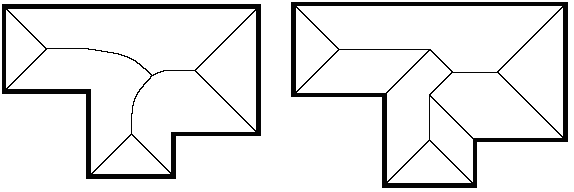
\includegraphics[width=15cm]{med.png}
\end{center}
\caption{(a) Medial axis vs (b) esqueleto recto.}
\end{figure}

La estructura arb\'{o}rea del esqueleto recto implica que, si $P$ es un pol%
\'{\i}gono no convexo, $S(P)$ tiene menor tama\~{n}o combinatorial que el
medial axis de $P$. Aunque los dos representan un \'{a}rbol, este \'{u}ltimo
tiene que distinguir entre partes rectas de arcos y curvas. M\'{a}s expl%
\'{\i}citamente, si $P$ tiene $r$ v\'{e}rtices reflexivos entonces $S(P)$
tiene $2n-3$ arcos mientras que el eje medio de $P$ da lugar a $2n+r-3$
arcos de los cuales $r$ son curvas parab\'{o}licas.

El medial axis, como caso particular del diagrama de Voronoi, est\'{a}
determinado sobre un modelo de distancia. El esqueleto recto no es definido
usando una funci\'{o}n de distancia, por el contrario est\'{e} se encuentra
determinado por un apropiado proceso de encogimiento del pol\'{\i}gono. El
esqueleto recto puede ser \'{u}til en aplicaciones del medial axis como, por
ejemplo, en el reconocimiento de formas \cite{motor}.

\section{Propiedades b\'{a}sicas}

En esta secci\'{o}n mencionaremos algunas de las propiedades elementales del
esqueleto recto, $S(P)$. Con el prop\'{o}sito de distinguirlos de los
elementos de $P$, a los cuales se les llamar\'{a} v\'{e}rtices y aristas, den%
\'{o}tese por nodos y arcos los elementos de $S(P)$ que no forman parte de $%
P $. Cada arista $e$ de $P$ recorre una cierta \'{a}rea a la cual se le
denominar\'{a}, en concordancia con la literatura, cara de $e$.

Los nodos de $S(P)$ pueden tener un grado mayor que tres. Por lo general,
esto tiene lugar cuando algunos eventos ocurren simult\'{a}neamene. Se puede
citar, por ejemplo, el caso en el que se est\'{e} reduciendo un pol\'{\i}%
gono regular. En ausencia de esta situaci\'{o}n, se cumple que $S(P)$ da
lugar a $n-2$ nodos y $2n-3$ arcos exactamente, como se demuestra en el
siguiente lema.

\begin{lemma}
$S(P)$ es un \'{a}rbol y consiste en exactamente $n$ caras conectadas, $n-2$
nodos y $2n-3$ arcos.
\end{lemma}

\begin{proof}
La construcci\'{o}n de una cara $f(e)$ comienza en su arista, $e$, de $P$. $%
f(e)$ no puede ser dividida a\'{u}n cuando e parezca serlo. La construcci%
\'{o}n de $f(e)$ est\'{a} completa cuando (cada parte de) $e$ ha sido
reducida a cero. Como $e$ no puede reaparecer otra vez, $f(e)$ es conexa, y $%
S(P)$ es ac\'{\i}clico. Lo que significa que $S(P)$ es un \'{a}rbol con $n$ v%
\'{e}rtices de $P$ como hojas y tiene $n-2$ nodos y $2n-3$ arcos. 
\end{proof}

Dos tipos de arcos de $S(P)$ se pueden distinguir. Cada arco viene dado por
un segmento de la recta bisectriz de dos aristas $e$ y $e^{\prime }$ de $P$ o,
m\'{a}s precisamente, de las l\'{\i}neas $l(e)$ y $l(e^{\prime} )$ que
soportan estas aristas. N\'{o}tese que la intersecci\'on de las l\'ineas $l(e)$ y $%
l(e^{\prime} )$ determina dos ang\'ulos y por consiguiente dos bisectrices. La bisectriz relevante ser\'a singularizada de la
siguiente manera. Cada l\'{\i}nea $l(e)$ define un semiplano $h(e)$ que
contiene a $P$, es decir, $h(e)$ es el semiplano en el que se encuentra el interior de $P$ 
respecto a la arista $e$. Una de las bisectrices intersecta la cu\~{n}a $h(e)
$ $\cap$ $h(e^{\prime} )$ mientras que la otra la evita. Ll\'{a}mese a esta,
\emph{bisectriz} de las aristas $e$ y $e^{\prime }$ e ign\'{o}rese la otra
considerada. Un arco $a$ definido por esta bisectriz es denominado un arco
convexo o un arco reflexivo dependiendo de cuando la cu\~{n}a contenga a
ambas aristas $e$ y $e^{\prime} $ en su frontera o no.

Cada v\'{e}rtice convexo (reflexivo) de $P$ obviamente da lugar a un arco
convexo (reflexivo) de $S(P)$. Arcos convexos pueden conectar a
dos nodos de $S(P)$, esto es imposible para arcos reflexivos.

\begin{lemma}
Arcos reflexivos de $S(P)$ s\'olo emanan de v\'ertices reflexivos de $P$.
\end{lemma}

\begin{proof}
Sea $vu$ un arco emanado por alg\'un v\'ertice $v$ de $P$. Entonces $u$ es un nodo que corresponde a un evento de arista o a un evento de divisi\'on. Es suficiente mostrar que, despu\'es del evento, $S(P)$ contin\'ua en $u$ con arcos convexos solamente. 

En el primer caso, sea $vw$ la arista desvanecida. Dado que el arco $wu$ se encuentra con $vu$ en $u$, $u$ es un v\'ertice convexo del pol\'igono encogido en el momento que el evento toma lugar. En el otro caso, el pol\'igono se divide en $u$. Es obvio que, en ese momento $u$ es un v\'ertice convexo de ambos nuevos pol\'igonos.

En conclusi\'on, cada nuevo v\'ertice generado durante el proceso de encogimiento es convexo. Entonces los arcos que parten de $u$ son convexos tambi\'en.
\end{proof}

Una buena propiedad de $S(P)$ es que particiona a $P$ en pol\'igonos mon\'otonos. Cada uno de estos pol\'igonos representa la cara de una arista y es mon\'otono en la direcci\'on de esta \'ultima \cite{AA}. 


\section{C\'omputo del esqueleto recto}

El primer algoritmo mostrado por Aichholzer \cite{AA} computa el esqueleto recto
de un pol\'{\i}gono simple de $n$ v\'ertices en un tiempo dado por $O(n^2\log{n})$
simulando, de forma discreta, el proceso de encogimiento. M\'{a}s adelante
Aichholzer y Aurenhammer \cite{AA2} lo generalizaron para figuras poligonales en el
plano y disminuyeron la complejidad espacial a $O(n)$. Adem\'as
mostraron que, a diferencia del medial axis, el esqueleto recto no puede ser descrito utilizando un modelo de distancia . Esta es la raz\'{o}n por la
cual, las bien desarrolladas t\'{e}cnicas en geometr\'{\i}a computacional,
tales como los diagramas de Voronoi concretos y los abstractos, no son
aplicables en el c\'{o}mputo de $S(P)$. 

En 1997, Eppstein y Erickson \cite{EE} encontrar\'on el primer algoritmo subcuadr\'{a}tico con un tiempo de ejecuci\'on dado por $O(n^{17/11+\epsilon})$ y similar tiempo de complejidad espacial. Tambi\'{e}n ellos presentaron un algoritmo sensitivo al n\'{u}mero de v\'{e}%
rtices reflexivos involucrados con un tiempo de complejidad dado por $O(n^{1+\epsilon}+
n^{8/11+\epsilon}r^{9/11+\epsilon})$, donde $r$ es el n\'{u}mero de v\'{e}rtices reflexivos del pol\'{\i}gono.

Es poca la publicidad disponible en la literatura sobre los detalles de implementaci\'on del algiritmo de construcci\'on del esqueleto recto. Esta es la raz\'on por la cual, se realiz\'o una sencilla implementaci\'on basada en una simulaci\'on discreta del proceso de contracci\'on o dilataci\'on de un pol\'igono simple. Los detalles de la misma son expuestos a continuaci\'on.\bigskip

La estructura de almacenamiento b\'{a}sica utilizada por el algoritmo es una 
\emph{lista circular de \'{a}rboles} (LCA) doblemente enlazada. El esqueleto recto, $S(P)$
presenta una estructura arb\'{o}rea, por lo que, en esta secci\'{o}n se hace
referencia a $S(P)$ como \'{a}rbol. Cada \'{a}rbol de la lista representar%
\'{a} un posible sub\'{a}rbol de $S(P)$. $S(P)$ es construido mediante un
apropiado proceso de mezcla de \'{a}rboles. En el momento en que la
cardinalidad de la LCA sea uno, se habr\'{a} obtenido el \'{a}rbol
correspondiente al esqueleto recto hacia el interior del pol\'{\i}gono.

En principio tendremos almacenados en la LCA $n$ \'{a}rboles, constituidos
por los v\'{e}rtices de $P$. Estos \'{a}rboles formar\'{a}n las hojas del 
\'{a}rbol $S(P)$. Cada sub\'{a}rbol de $S(P)$ tendr\'{a} asosiado dos aristas de $P$ y un
arco que represente la bisectriz formada por dichas aristas. La mezcla entre
dos \'{a}rboles es detallada a continuaci\'{o}n.

Sup\'{o}ngase que se est\'{e} an\'{a}lizando la mezcla de un arbol $A_{i}$
con sus respectivos adyacentes $A_{i-1}$ y $A_{i+1}$. Si el arco $b_{i}$
correspondienete a $A_{i}$ se intersecta con sus respectivos arcos
adyacentes $b_{i-1}$ y $b_{i+1}$. S\'{o}lo se tendr\'{a} en cuenta el punto
de intersecci\'{o}n m\'{a}s cercano al nodo ra\'{\i}z de $A_{i}$. Ver Figura
2.3(a). Esta intersecci\'{o}n, si existe, es referenciada como intersecci\'{o}n
v\'{a}lida. Pudiera suceder que ambas intersecciones se prod{u}jesen en un
mismo punto, en este caso ambas son v\'{a}lidas y tratadas secuencialmente. 

\begin{figure}[htbp]
\begin{center}
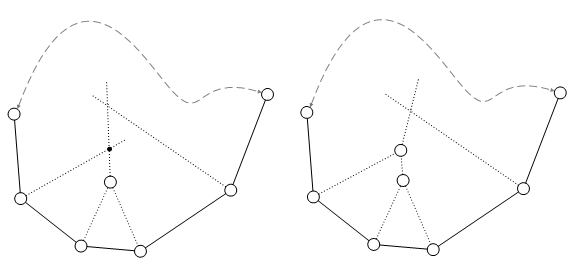
\includegraphics{inter4.png}
\end{center}
\caption{(a) Intersecci\'on v\'alida en negro y (b) \'arbol resultante de una mezcla de \'union.}
\end{figure}

La mezcla solo tendr\'{a} lugar entre dos \'{a}rboles $A_{1}$\ y $A_{2}$
adyacentes. Denotemos por $a_{1}$ y $a_{2}$ los arcos correspondientes a $%
A_{1}$\ y $A_{2}$ respectivamente. En correspondencia con los eventos
analizados tendremos dos tipos mezcla. 

El evento de arista representa una mezcla en la que los \'{a}rboles $A_{1}$
y $A_{2}$ se funden formando un nuevo \'{a}rbol $A$ teniendo por hijos a los 
\'{a}rboles $A_{1}$ y $A_{2}$. Esta mezcla ser\'{a} llamada \emph{mezcla de
uni\'{o}n}. Esto implica que la intersecci\'{o}n entre $a_{1}$ y $a_{2}$ es v\'{a}%
lida. $A_{1}$ y $A_{2}$ son remplazados en la LCA por $A$, disminuyendo su
cardinalidad en uno. Ver Figura 2.3(b).

Ll\'{a}mese ladera de un \'{a}rbol al camino simple desde su ra\'{\i}z hasta
la primera o la \'{u}ltima de sus hojas.

El evento de divisi\'{o}n es representado, sin p\'{e}rdida de generalidad,
por la mezcla entre $A_{1}$ y un sub\'{a}rbol de $A_{2}$, a este \'{u}ltimo
llam\'{e}sele $A_{s}$. Este caso es referido como \emph{mezcla de corte}.
Sea $C(A_{s})$ el conjunto de los nodos de la ladera de $A_{s}$ pr\'{o}xima
a $A_{1}$ y $C(A_{2})$ el conjunto de los nodos de la ladera de $A_{2}$ tambi%
\'{e}n pr\'{o}xima a $A_{1}$. Entonces $C(A_{s}) \subset C(A_{2})$. De la
misma manera que en la mezcla de uni\'on, $A_{1}$ y $A_{s}$\ se funden. Los sub%
\'{a}rboles contenidos en $A_{2}$, hijos de los nodos pertenecientes a $%
C(A_{2})-C(A_{s})$ son reinsertados en la LCA. Esta mezcla provoca un
aumento en la cardinalidad de la LCA. Ver Figura 2.4.

\begin{figure}[htbp]
\begin{center}
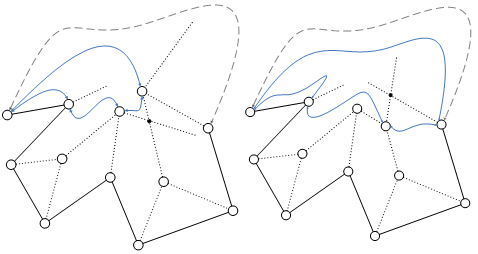
\includegraphics{corte1.jpg}
\end{center}
\caption{(a) Mezcla de corte y (b) consecuencias de esta en la LCA.}
\end{figure}

En ambos tipos de mezcla pudiera suceder que el \'{a}rbol $A_{1}$ cortas\'{e}
a $A_{2}$ por sobre un nodo $n$, lo cual refleja que varios eventos est\'{a}n
sucediendo de forma simult\'{a}nea. En estos casos se procede de forma an%
\'{a}loga, seg\'{u}n el tipo de mezcla que se est\'{e} tratando, con la
excepci\'{o}n de que no se crea un nuevo nodo. El nodo $n$ por sobre el cual pasa
el corte, pasa a ser la ra\'{\i}z del nuevo \'{a}rbol que tendr\'a como hijo a $A_{1}$. $A_{1}$ estar\'a como primer o \'ultimo hijo en dependencia de la posici\'on relativa de $A_{1}$ con respecto a $A_{2}$. Ver Figura 2.5.

\begin{figure}[htbp]
\begin{center}
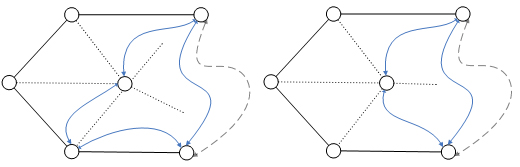
\includegraphics{nodo1.jpg}
\end{center}
\caption{(a) Eventos simultaneos y (b) consecuencias de estos en la LCA.}
\end{figure}

Un \'{a}rbol reflexivo es un \'{a}rbol que tiene un arco reflexivo conectado
a su ra\'{\i}z. En el algoritmo que se expone se ha hecho el siguiente
presupuesto.

\begin{conjecture}
Una mezcla de corte s\'olo es inducida por un \'arbol reflexivo.  
\end{conjecture}

El presupuesto anterior discrimina, de antemano, el tipo de mezcla que se
producir\'{a}. O sea, s\'{o}lo cuando se est\'e en presencia de un \'{a}rbol
reflexivo, se realizar\'{a} una b\'{u}squeda de la posible intersecci\'{o}n
de su arco bisectriz con los arcos contenidos en la ladera correspondiente de sus
respectivos \'arboles adyacentes. 

En el algoritmo se ha hecho uso de una cola de prioridad como estructra auxiliar. Esta cola es implementada utilizando un Heap \cite{IA}. En ella se almacenar\'an las intersecciones que ocurran entre las bisectrices del pol\'igono. La prioridad es dada a la intersecci\'on que cumpla que la distancia, entre este punto de intersecci\'on y una de las aristas involucradas en el c\'omputo de la bisectriz en la que este punto se encuentre, sea menor.   

\begin{flushleft}
\bfseries{Algoritmo para el c\'omputo del esqueleto recto de un pol\'igono simple. }
\end{flushleft}

\begin{itemize}
\item[1)] Inicializaci\'{o}n:

\begin{itemize}
\item[(a)] crea con los v\'{e}rtices dados $V_{1},V_{2}\ldots ,V_{n}$ un 
\'{a}rbol para luego almacenar cada \'{a}rbol en la LCA. Tendremos en este
momento $n$ \'{a}rboles activos.\qquad 

\item[(b)] por cada \'{a}rbol $A_{i\text{,}}$\ almacenado en la LCA, a\~{n}%
adir dos referencias a las aristas incidentes (en este momento los \'{a}%
rboles son los vertices del pol\'{\i}gono) y computar la bisectriz .

\item[(c)] para cada \'{a}rbol$\ A_{i}$ calcular la intersecci\'{o}n v\'{a}%
lida de la bisectriz con las bisectrices de los \'{a}rboles adyacentes $%
A_{i-1}$ y $A_{i+1}$ y (si existe) almacenarla dentro de una cola de
prioridad de acuerdo con la distancia a la l\'{\i}nea soporte de la arista .
Para cada intersecci\'{o}n almacenar tambi\'{e}n dos referencias a los \'{a}%
rboles $A_{l}$ y $A_{r}$, lo que significa dos or\'{\i}genes de las
bisectrices que crean el punto de intersecci\'{o}n $I$. Estos son necesarios
para la identificaci\'{o}n adecuada de las aristas $e_{l}$ y $e_{r}$ durante
el c\'{o}mputo de las bisectrices en pasos posteriores del algoritmo.
Guardar el tipo de mezcla (mezcla por uni\'{o}n o mezcla por corte). \qquad 
\end{itemize}

\item[2)] Mientras la cola de prioridad de los puntos de intersecci\'{o}n
tenga m\'{a}s de dos intersecciones hacer:

\begin{itemize}
\item[(a)] extraer el punto de intersecci\'{o}n $I$\ del tope de la cola de
prioridad

\item[(b)] si los \'{a}rboles apuntados por $I$ est\'{a}n marcados como
procesados o si alguno est\'{a} marcado y la intersecci\'{o}n no es v\'{a}%
lida, entonces continuar en el paso 2 \qquad 

\item[(c)] Si la intersecci\'{o}n es producida por una mezcla de uni\'{o}n.

\begin{itemize}
\item[i] marcar los \'{a}rboles $A_{l}$ y $A_{r}$ (referenciados por $I$)
como procesados

\item[ii] crear un nuevo \'{a}rbol $A$ teniendo como hijos a $A_{l}$ y $A_{r}
$. Insertar $A$\ en la LCA, lo que significa conectarlo con el predecesor de 
$A_{l}$ y el sucesor de $A_{r}$

\item[iii] conectar el nuevo \'{a}rbol $A$ con las apropiadas aristas $e_{l}$
y $e_{r}$ (apuntadas por los \'{a}rboles $A_{l}$ y $A_{r}$ respectivamente)

\item[iv] para el nuevo \'{a}rbol $A_{i}$ creado a partir de $I$, computar: 

\begin{itemize}
\item una bisectriz $b_{i}$ entre las aristas $e_{l}$ y $e_{r}$

\item la intersecci\'{o}n v\'{a}lida $I_{v}$ (si existe) de $b_{i}$ con sus
bisectrices adyacentes analizando, en caso de que $A_{i}$ o alguno de sus 
\'{a}rboles adyacentes fuese reflexivo, la intersecci\'{o}n de todos los
arcos de la ladera de $A_{i-1}$ y $A_{i+1}$ pr\'{o}xima a $A_{i}$, con $b_{i}$

\item almacenar $I_{v}$ (si existe) en la cola de prioridad y el el tipo de
mezcla que produjo
\end{itemize}
\end{itemize}

\item[(d)] En caso contrario, si la intersecci\'{o}n es producida por una
mezcla de corte y el corte se produce con $A_r$ (el pseudoc\'{o}digo para el
caso en que el corte hubier\'{a} sido a $A_{l}$ es sim\'{e}trico) 

\begin{itemize}
\item[i] insertar cada sub\'{a}rbol, hijo de los nodos de la ladera, ver
Figura 2.4, en la LCA como predecesores del \'{a}rbol contenedor de $A_{r}$, adem%
\'{a}s de remarcarlos como no procesados

\item[ii] quitar al \'{a}rbol contenedor de $A_{r}$ de la LCA.  

\item[iii] crear un nuevo \'{a}rbol $A$\ a\~{n}adiendo como hijos a $A_{l}$
y $A_{r}$

\item[iv] remplazar $A_{l}$ por $A$ en la LCA

\item[v] computar la bisectriz de $A$

\item[vi] para el nuevo \'{a}rbol A y los subarboles reci\'{e}n reinsertdos
en la LCA computar la intersecci\'{o}n v\'{a}lida con sus respectivos
adyacentes y almacenarlas en la cola de prioridad asi como, el tipo de
mezcla correspondiente a cada una de ellas
\end{itemize}
\end{itemize}

\item[3)] Teniendo dos \'{a}rboles $A_{1}$ y $A_{2}$\ en la LCA a\~{n}adir
como hijo de $A_{1}$ a $A_{2}$, si $A_{1}$ no representa un v\'{e}rtice, en
caso de serlo hacer la operaci\'{o}n contraria (ambos no pueden representar v%
\'{e}rtices ya que un pol\'{\i}gono tiene al menos tres v\'{e}rtices).

\item[4)] Devolver el \'{a}rbol resultante. FIN.
\end{itemize}
\bigskip

El algoritmo antes expuesto puede ser f\'{a}cilmente modificado para tratar
el c\'{o}mputo del esqueleto recto hacia el exterior del pol\'{\i}gono.
Simplemente el resultado, en lugar de ser un \'{u}nico \'{a}rbol, como es el
caso del esqueleto recto en su interior, ser\'{a} una LCA. Lo anterior se
debe a la ausencia de intersecci\'{o}n de arcos por lo que tendremos \'{a}%
rboles que nunca lleguen a mezclarse.

En este caso y en particular para el algoritmo antes presentado, nos
encontramos con la cola de prioridad vac\'{\i}a por lo que se devuelve la
LCA presente en ese momento. Otra particularidad que se tuvo en cuenta, en
el caso en que se quiera obtener el esqueleto recto hacia el exterior del pol%
\'{\i}gono, fue la aisignaci\'{o}n a cada \'{a}rbol en la LCA de un padre
fict\'{\i}cio infinito sobre la bisecriz definida por su ra\'{\i}z. Esto se
realiz\'{o} en consecuencia con que, cada cara de este tipo de esqueleto, va
a ser abierta. Adem\'{a}s como se ver\'{a} en el pr\'{o}ximo cap\'{\i}tulo
esto es conveniente en el c\'{a}lculo siguiente, ya que permite la obtenci\'on del conjunto resultado para ambos casos en un mismo algoritmo. Ver Figura 2.6.

\begin{figure}[htbp]
\begin{center}
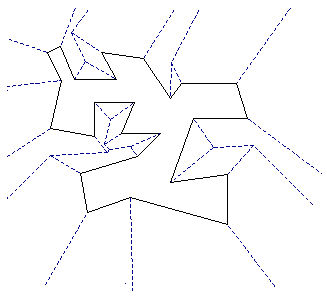
\includegraphics{fuera1.png}
\end{center}
\caption{Esqueleto hacia el exterior del pol\'igono.}
\end{figure}

Los pol\'{\i}gonos convexos son particularmente tratados en la construcci%
\'{o}n del esqueleto recto ya sea hacia el interior o exterior de $P$. La no
presencia de v\'{e}rtices reflexivos en ellos, y por ende de \'{a}rboles
reflexivos, elimina, seg\'{u}n el presupuesto visto, la posibilidad de que
se produzca una mezcla de corte. En el primer caso la construcci\'{o}n del 
\'{a}rbol se hace gradual. En el otro caso, obtenemos el resutado de forma
directa ya que las bisectrices de los v\'{e}rtices del pol\'igono no se intersectan, por lo
que el resultado radica en una LCA con exactamernte $n$ \'{a}rboles
constituidos estos v\'{e}rtices.

\begin{flushleft}
\bfseries {\normalsize{An\'alisis}}
\end{flushleft}

Por conveniencia, se ha separado el an\'{a}lisis del algoritmo en dos casos: para pol\'{\i}%
gonos convexos y no convexos. La complejidad espacial, en cualquiera de
estos casos, es dada en $O(n)$ ya que esta depende linearmente del n\'{u}%
mero de nodos involucrados en $S(P)$, que a lo sumo es $n-2$, en adici\'{o}n
de los v\'{e}rtices del pol\'{\i}gono que forman las hojas del esqueleto
recto.

Si el pol\'{\i}gono $P$ es convexo y $S(P)$ es construido hacia el exterior
de $P$ el tiempo de complejidad viene dado por $O(n)$ ya que no se producen
intersecciones. En este caso, cuando la construcci\'{o}n de $S(P)$ se
realiza hacia el exterior, el tiempo de complejidad que se expone est\'{a}
basado en el \textbf{Presupuesto 1.4.1}. Esta complejidad est\'{a} dada en $O(n\log n)$ ya que cada intersecci\'{o}n encontrada es almacenada en la cola de prioridad en un
tiempo logar\'{\i}tmico. Se puede estabecer una correspondencia lineal entre
el n\'{u}mero de intersecciones analizadas por el algoritmo y el n\'{u}mero
de v\'{e}rtices del pol\'{\i}gono. 

Hasta este momento, no se ha encontrado el orden de complejidad del
algoritmo para los casos en que se traten pol\'{\i}gonos no convexos. En la pr\'actica se puede comprobar que este es eficiente y alcanza su punto de parada. 

%%%%%%%%%%%%%%%%%Fin de esqueleto
%%%%%%%%%%%%%%%%%%%%%Inicio de paralelas
\chapter{Las paralelas}

En este cap\'{\i}tulo se propone un m\'{e}todo eficiente para la obtenci\'{o}%
n, a partir del esqueleto recto, del conjunto de pol\'{\i}gonos resultado
del problema planteado. En el dise\~{n}o expuesto, esto equivale a encontrar
una funci\'{o}n que dada una lista circular de \'{a}rboles LCA devuelva el
adecuado conjunto. 

\section{Relaci\'{o}n entre las caras del esqueleto y las aristas de la
poligonal resultante. }

El esqueleto recto $S(P)$ se encuentra determinado, de manera un\'{\i}voca,
por $n$ caras. Cada arista $e$ define una \'{u}nica cara en $S(P)$ de la
cual forma parte. Las caras de $S(P)$ se encuentran conectadas. Cada cara  $%
f(e)$ representa un pol\'{\i}gono mon\'{o}tono en la direcci\'{o}n de $e$
\cite{AA}. $f(e)$ representa el \'{a}rea recorrida por $e$ cuando el pol\'{\i}%
gono original $P$ es contraido o dilatado. Cada nodo de $S(P)$ define un arco del mismo con excepci\'{o}n de su ra\'{\i}z. $f(e)$ est\'{a} determinada por
las intersecciones producidas entre $e$ y el resto de las aristas de $P$, al
ser todas trasladadas a una misma velocidad. Ver \textbf{Lema 2.3.1}.  

Los arcos de una cara de $S(P)$ se encuentran reflejados en el \'{a}rbol $%
S(P)$ por los arcos involucrados en el camino simple desde un v\'{e}rtice
hoja hasta la siguiente (adyacente) hoja. Los arcos de $S(P)$, involucrados en $%
f(e)$, son los involucrados en el recorrido simple desde un extremo de $e$
hasta el otro. Ver Figura 3.1.

\begin{figure}[htbp]
\begin{center}
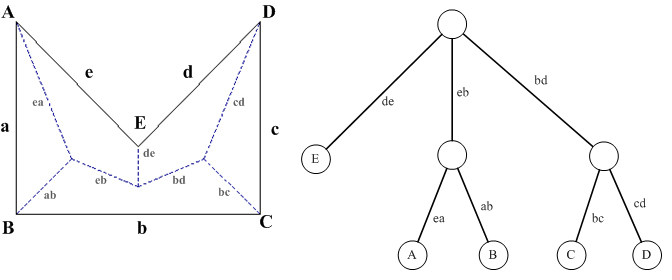
\includegraphics{arbol.jpg}%[width=15cm]
\end{center}
\caption{(a) Vista geom\'etrica de $S(P)$ y (b) vista arb\'orea de $S(P)$}
\end{figure}

Sea $p(e)$ la l\'inea paralela a la arista $e$ que se encuentra a distancia $d$%
. El algoritmo que se presentar\'{a} efect\'{u}a un recorrido por el \'{a}%
rbol $S(P)$ o, m\'{a}s espec\'{\i}ficamente, por cada cara de $S(P)$, h\'allando las intersecciones de $p(e)$ con cada uno de los arcos que conforman $f(e)$. 

El ser la cara $f(e)$ un pol\'{\i}gono garantiza que $p(e)$ interecta $f(e)$ en una cantidad par de arcos. Sea $J(e)$ el conjunto de itersecciones
entre $p(e)$ y cada uno de los arcos de $f(e)$. Entonces, si $|J(e)| = \emptyset$, la
arista $e$ no va a estar reflejada en la poligonal resultante. Formalmente dicho,
ninguna arista en la poligonal resultante, va a estar relacionada con $e$.

La cara $f(e)$ es convexa si el desplazamiento de la arista $e$ no se vi\'o interrumpido por un arco reflexivo o un arco convexo, en el caso de que la construcci\'on de $S(P)$ haya sido hacia el exterior de $P$. Si $f(e)$ es convexa, entonces $e$ est\'a en correspondencia, a lo sumo, con un \'{u}nico segmento en la poligonal resultante, $J(e)=\emptyset \vee \left|J(e)\right|=1$.

El caso en que $f(e)$ no sea convexa es debido a que al menos un v\'{e}rtice
reflexivo (convexo si $S(P)$ se trata hacia el exterior) colision\'{o} a la
arista $e$ dividi\'{e}ndola; $e$ tuv\'{o} participaci\'{o}n en al
menos un evento de divisi\'{o}n. Esto provoca, tambi\'{e}n en dependencia de
la distancia, que $J(e) = \emptyset \vee \left| J(e) \right| \geq 2$, lo cual significa que a $e$ le
corresponden, al menos, un par de segmentos en la poligonal resultante. Ver
Figura 4. Es evidente que la $\left| J(e) \right|$ es par.

Cuando se pretende obtener la poligonal resultante de una dilataci\'{o}n del
pol\'{\i}gono se estar\'{a} trabajando con un esqueleto hacia el exterior
del mismo. Esto implica que existir\'{a}n caras abiertas. Los arcos que
conforman estas caras est\'{a}n representados en la LCA por los arcos de
un par de laderas vecinas. Ver Figura 3.2.  En caso que se tenga un \'{u}nico 
\'{a}rbol $A$ ($S(P)$ en el interior de $P$), el \'{a}rbol siguiente de $A$
es el propio $A$ y los arcos de una de sus caras son obtenidos recorriendo
cada una de sus laderas. Ver Figura 3.1.

\begin{figure}[htbp]
\begin{center}
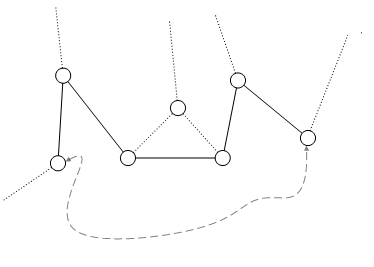
\includegraphics{cara.jpg}%[width=15cm]
\end{center}
\caption{Arcos que conforman la cara abierta}
\end{figure}

Es obvio que, cada vez que $p(e)$ entre en una cara abierta tendr\'{a} que
salir de esta.

\section{C\'{o}mputo del conjunto de pol\'{\i}gonos }

Con el objetivo de lograr una mayor legibilidad y f\'acil exposici\'on se realizar\'a el c\'omputo de las paralelas en dos procedimientos. Primero se mostrar\'a un procedemiento de recorrido de la LCA de acuerdo con la cara que se est\'e analizando. Luego se expondr\'a el algoritmo que construya la poligonal resultante a medida en que hace dicho recorrido. 

Se marcar\'an las caras analizadas para no caer en un ciclo infinito. Esto es posible ya que el conjunto de caras se encuentra conectado.
\bigskip    

\textbf{Procedimiento de recorrido de una hoja $h$ hasta la siguiente hoja $h'$. Esto equivale a devover los arcos de una cara.}
\begin{itemize}
	\item[1)]	Si $h$ esta marcada fin del recorrido. En este punto se est\'a sobre una hoja de $S(P)$ por lo que, en el momento de inicio, se estar\'a comenzando una cara y en el punto de parada se estar\'a cerrando otra. En cualquier otro momento que se llegue a este punto se estar\'an haciendo las dos cosas. 
	\item[2)] Si $h$ es \'ultimo hijo	
\begin{itemize}
	\item Hacer $n \leftarrow h$
	\item Mientras $n \neq$ Ra\'iz$(S(P))\wedge n$ es \'ultimo hijo hacer $n \leftarrow $ Padre$(n)$
	%\item Hacer $n \leftarrow $ Padre$(h)$ mientras $n \neq$ Ra\'iz$(S(P))\wedge n$ es \'ultimo hijo
	\item Si $n =$ Ra\'iz$(S(P))$ 
\begin{itemize}
	\item hacer $n \leftarrow$ PrimerHijo$(n)$ mientras $n$ no es hoja. Ir al paso 1.
\end{itemize}		
	\item En caso contrario
\begin{itemize}
	\item $n \leftarrow$ Pr\'oximoHermano$(n)$
	\item Hacer $n \leftarrow$ PrimerHijo$(n)$ mientras n no sea hoja. Ir al paso 1.
\end{itemize}
\end{itemize}
	\item[3)] Si $h$ no es \'ultimo hijo	
\begin{itemize}
	\item $n \leftarrow$ Pr\'oximoHermano$(n)$
	\item Hacer $n \leftarrow$ PrimerHijo$(n)$ mientras n no sea hoja. Ir al paso 1.  
	
\end{itemize} 
\end{itemize}
\bigskip
\textbf{Contruci\'on de la poligonal resultante dado S(P) y una distancia $\delta$}
\begin{itemize}
	\item [(1)]Crear una pila $S$ inicialmente vacia.
	\item [(2)]Para cada cara $f(e)$ del recorrido c\'omputar la linea $p(e)$ paralela a la arista e y a distancia $\delta$.
	\item [(3)]Para cada arco a involucrado en el recorrido de $f(e)$ hacer
	\begin{itemize}
	\item [$\triangleright$]c\'omputar el punto de intersecci\'on $pt$ entre $p(e)$ con $a$. Si $pt$ no existe continuar en el paso (3). 
	\item [$\triangleright$]si $S$ esta vac\'ia almacenar $pt$ en $S$
	\item[$\triangleright$]si en el tope de $S$ hay un punto $t$ remplazarlo por un segmento con inicio en $t$ y final en $pt$. En este momento se forma un segmento en $f(e)$.
	\item[$\triangleright$]si en el tope de $S$ hay un segmento $seg$ entonces si $pt$ es igual al punto final de $seg$ remplazar seg por una poligonal constituida por ese segmento. En este momento se pasa para una nueva cara se va a construir una poligonal. En caso contrario almacenar $pt$ en $S$. En este caso la cara no es convexa y va a tener en su interior m\'as de un segmento.
	  \item[$\triangleright$]si en el tope de $S$ hay una poligonal $pl$ entonces si $pt$ es igual al punto de inicio de $pl$ sacar la poligonal del tope de la pila y devolverla. Se cierra una poligonal y se agrega el poligono resultante al conjunto resultado. En caso contrario agregar $pt$ a $pl$
\end{itemize}
\item[(4)]El algoritmo termina cuando son recorridas todas las caras. 
	
\end{itemize}

\begin{flushleft}
\bfseries {\normalsize{An\'alisis}}
\end{flushleft}

El tiempo de complejidad del algoritmo est\'a determinado por el recorrido que se realiza sobre cada cara de $S(P)$. En vista de que, en este recorrido, se pasa por cada arco del \'arbol $S(P)$ dos veces y el n\'umero de arcos esta acotado por $2n - 3$ el tiempo de ejecuci\'on del algoritmo es $O(n)$.

La complejidad espacial esta acotada, en el peor caso por $r$, donde $r$ es el n\'umero de v\'ertices reflexivos del pol\'igono. Esto sucede cuando una cara no es convexa pudiendo contener, a lo sumo, $r$ segmentos en ella.

  
%%%%%%%%%%%%%%%%%%%%%%%%%Conclusiones
\newpage
\begin{flushleft}
\textbf{\Huge Conclusiones}
\end{flushleft}
\bigskip
\bigskip

Se ha presentado un algoritmo para el c\'omputo del conjunto de pol\'igonos, resultante del crecimiento o decrecimiento un pol\'igono mediante paralelas, habiendo fijado, previamente, una distancia. Adem\'as se discuten toda una serie de caracter\'isticas que evidencia la complejidad que se presenta en este problema.

Para el alcance del objetivo trazado, se realiz\'o una sencilla implementaci\'on del algoritmo de construcci\'on del esqueleto recto de un pol\'igono simple, cuyos detalles son expl\'icitamente mostrados. En complemento de esto, se presenta un algoritmo para la obtenci\'on del conjunto resultado a partir de dicho esqueleto.  

Como problema abierto, se encuentra la extensi\'on de este problema a una poligonal abierta. Esta extensi\'on se presenta como un problema similar en construcci\'on al problema de dilatar de un pol\'igono, tratado en este trabajo. Otro de los problemas a resolver consiste en obtener la complejidad computacional del expuesto algoritmo de construcci\'on del esqueleto recto, para el caso en que el pol\'igono original no sea convexo.

\addcontentsline{toc}{chapter}{Bibliograf\'ia}
\begin{thebibliography}{9}

\bibitem{AA}O. Aichholzer y F. Aurenhammer, D. Alberts, y B. Gartnert. A novel type of skeleton for polygons. \emph{The Journal of Universal Computer Science}, 1(1995), 752-761.%

\bibitem{IA}Thomas H. Cormen, Charles E. Leiserson, y Ronald L. Rivest. Introduction to Algorithms.

\bibitem{AA2}O. Aichholzer y F. Aurenhammer. Stright skeletons for general polygonal figures. \emph{Proc. 2nd Annu. Int'l. Computing and Combinatorics Conf}., 1996, 117-126. 

\bibitem{EE}D.Eppstein y J. Erickson. Raising roof, crashing cycles and playing pool: Applications of a data structure for finding pairwise interactions. \emph{Discrete Compt. Geom}., 22(1999), 569-592. 

\bibitem{motor}SW. Cheng y A. Vigneron. \emph{Motorcycle Graphs and Stright Skeletons}. 2001, 2005.  

\bibitem{} P. Felkel y S.Obdrzalek. Stright skeleton implementation. In \emph{Proc. 14th Spring Conf. Comp. Graphics}, 210-218, 1998.  

\end{thebibliography}


\end{document}
